The Component Diagram shown below describes the logical components of the system we are to develop, from a very high-level description on to a more detailed one. This diagram does not take into account the deployment phase, hence it doesn't describe the logical layer of the system in terms of the physical tiers where it is deployed. It also does not show the interfaces between the logical layer and the end users or the database, for simplicity %TODO do we have to add them?

	\subsubsection{High level components}
		\paragraph{} We shall show below the high level view of the logical components of the system and their interactions. Following the UML 1 notation, the dashed arrows represent dependencies between components, with the tail end component depending on the point end component (e.g. if \textit{A -> B}, then A \textit{depends on} B). 

		
		\begin{figure}[h]
			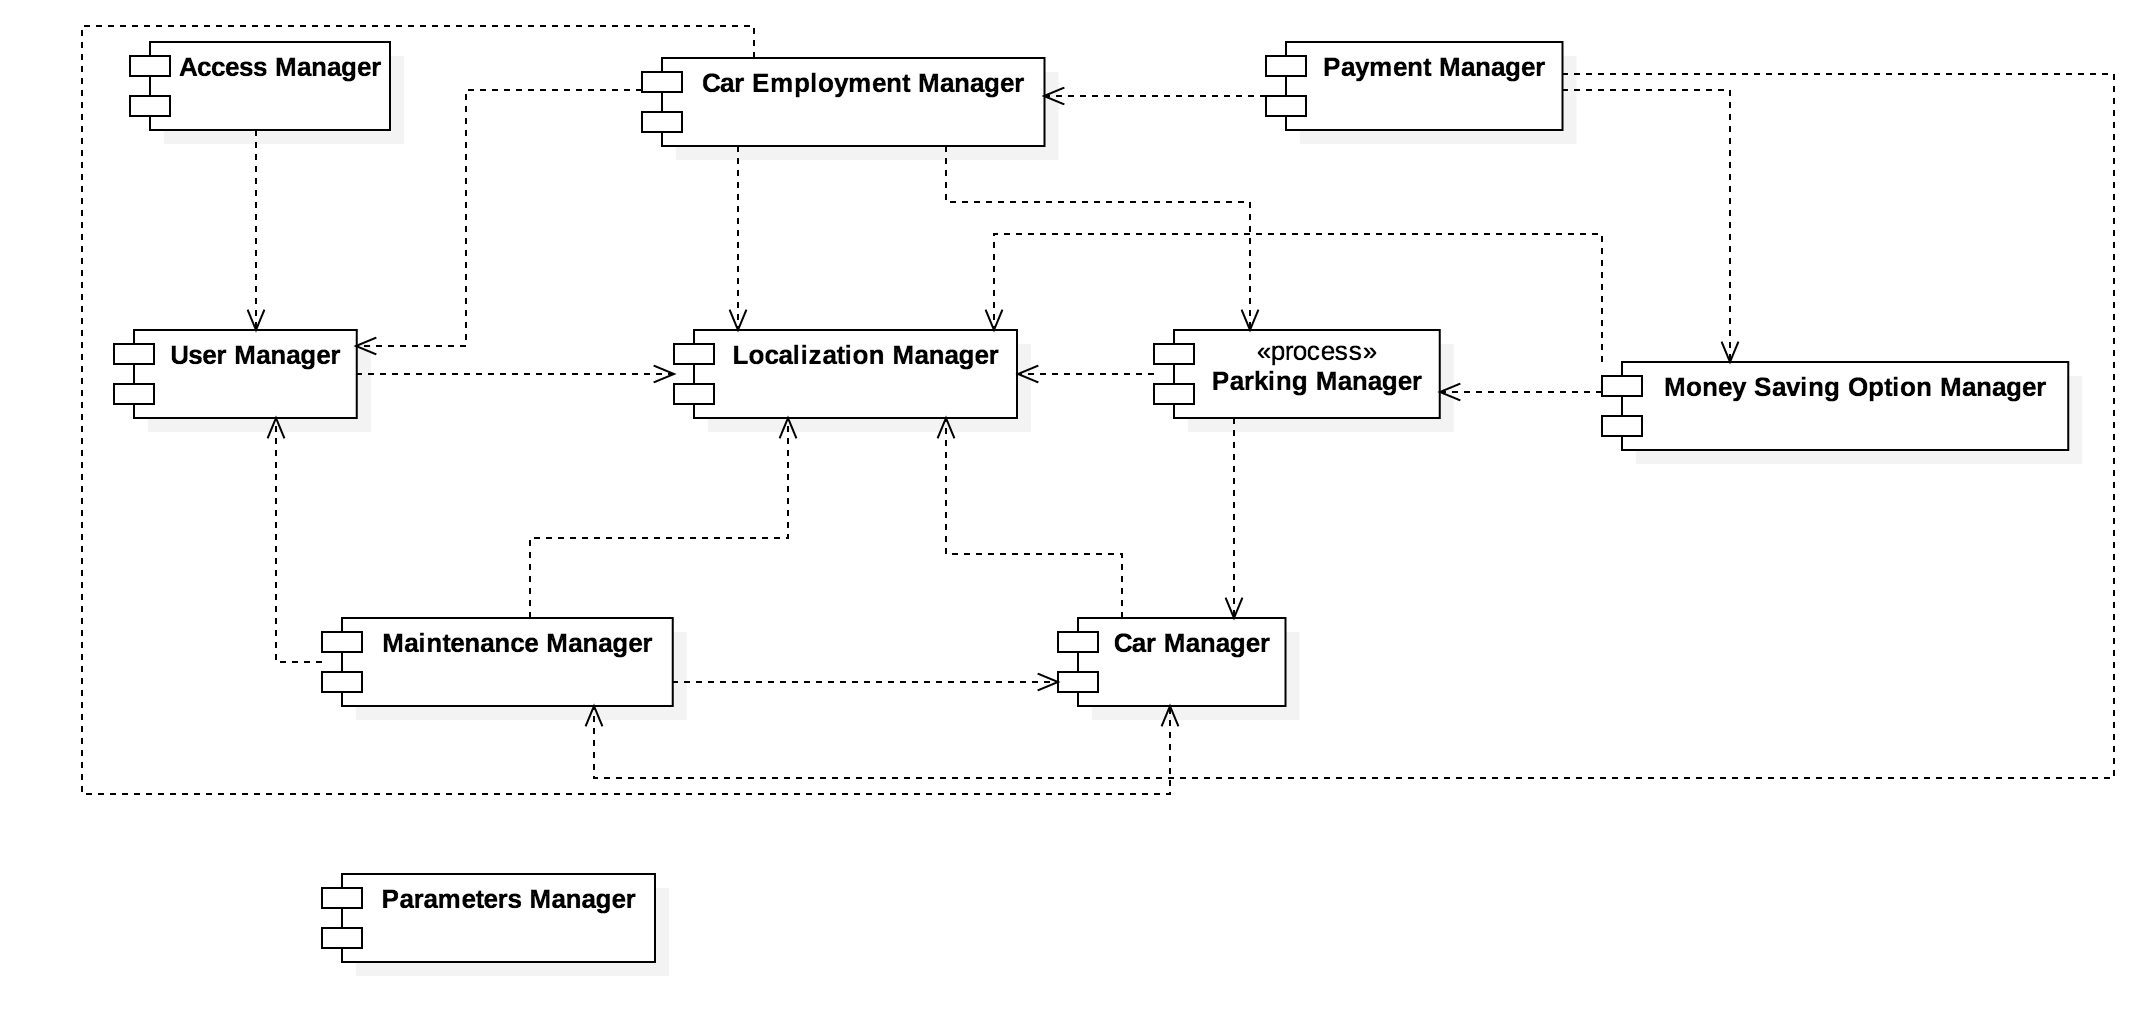
\includegraphics[scale=0.24]{img/component_diagrams/01_high_level_component_view.png}
		\end{figure}

	\subsubsection{Component view}
	
	
	
		\paragraph{Access Manager}
		
			\begin{figure}[h]
				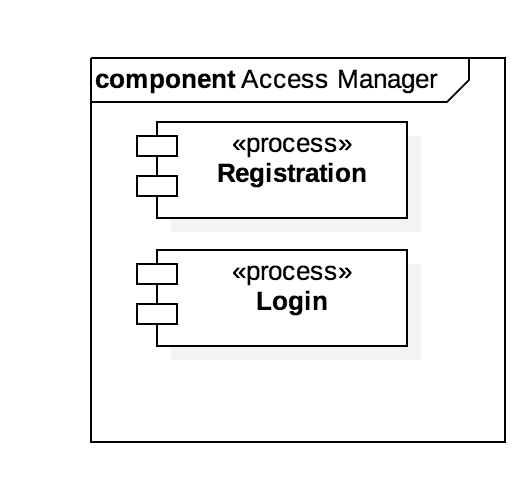
\includegraphics[scale=0.4, center]{img/component_diagrams/02_access_manager.png}
			\end{figure}
			
		\paragraph{}The Access Manager deals with the first interactions of a user or a guest with the system at the beginning of each session. Every further interaction with the system requires either a log in or the registration, both of which are managed by independent processes. The login interfaces with the User Handler to verify the validity of the login information and to allow the authenticated user to continue employing the system. Both processes also interface with the database.
		
		
		
		
		\paragraph{User Manager}
		
			\begin{figure}[h]
				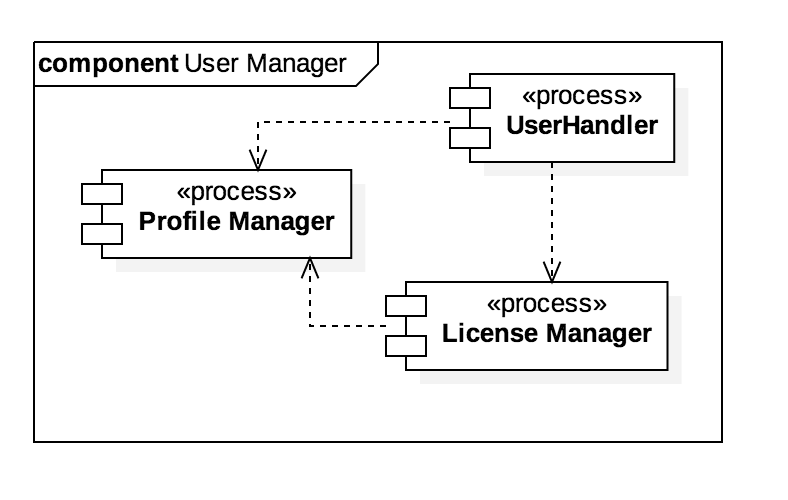
\includegraphics[scale=0.4, center]{img/component_diagrams/03_user_manager.png}
			\end{figure}
			
		\paragraph{} The User Manager manages all interaction that a registered user has with the rest of the system. The User Handler functions as an interface component between the user themselves and the system, and to be associated with a user needs to be linked to the Profile Manager. This latter component interfaces with the DBMS and controls the validity of all data in the user's profile and its changes; the exception to this is the driving license data, that is checked by the License Manager since it's a particularly critical piece of information. The Profile Manager also depends on the License Manager in that every time the user tries to reserve a car the Profile Manager asks the License Manager for the validity of the user's license. 
		
		
		\paragraph{Car Employment Manager}
		
			\begin{figure}[h]
				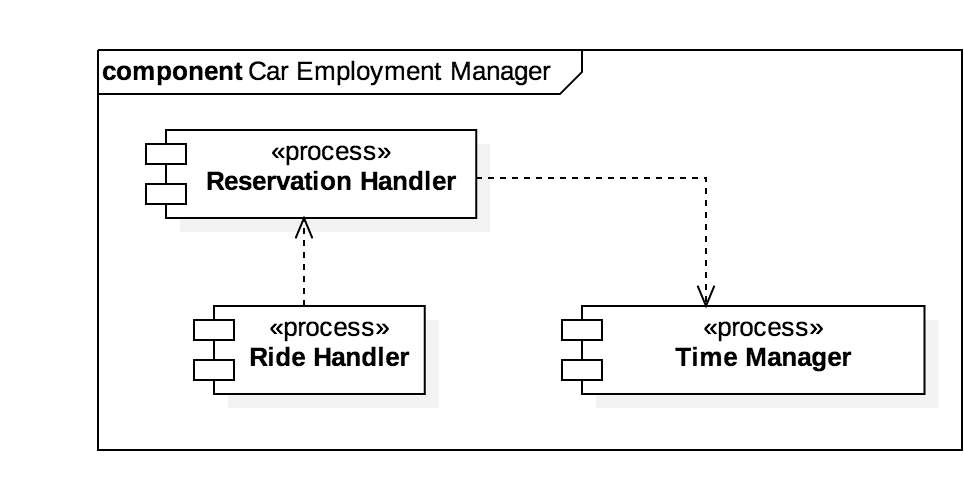
\includegraphics[scale=0.4, center]{img/component_diagrams/04_car_employment_manager.png} %TODO modify the image, a dependency is missing
			\end{figure}
			
		\paragraph{} The Car Employment Manager is one of the most important component of the system in terms of its core functionalities. It's composed of three processes: the first one, the Reservation Handler, has the task of dealing with reservations from a user and for an individual car. It blocks all other possible operations to that car until the user starts using it or the reservation expires. To keep track of the time, the Reservation Handler needs to interface with the Time Manager. This process is tasked with keeping track of the time periods necessary for the services to be offered: the expiration time for a reservation, the duration of a ride, the time window after a ride has finished. 
		The Ride Handler on the other hand depends on the Reservation Handler in that a car can be used only after a reservation. The Ride Handler is associated to a particular car and a particular user. It depends on the Time Manager to keep track of the duration of the ride. 